\subsection{Results using Soft Drop (from Suman)}
\begin{figure}[H]
    \begin{center}
        \includegraphics[width=0.7\textwidth]{Canv_jetecalbye.pdf}
        \caption{Fraction of jet energy deposited in ECAL (distribution has been normalized to unit area under curve)}
    \end{center}
\end{figure}
\begin{figure}[H]
    \begin{center}
        \includegraphics[width=0.7\textwidth]{Canv_jethcalbye.pdf}
        \caption{Fraction of jet energy deposited in HCAL (distribution has been normalized to unit area under curve)}
    \end{center}
\end{figure}
\begin{figure}[H]
    \begin{center}
        \includegraphics[width=0.7\textwidth]{Canv_jethovere.pdf}
        \caption{Ratio of jet energy deposited in HCAL with respect to the enrgy deposit in ECAL(distribution has been normalized to unit area under curve)}
    \end{center}
\end{figure}
\begin{figure}[H]
    \begin{center}
        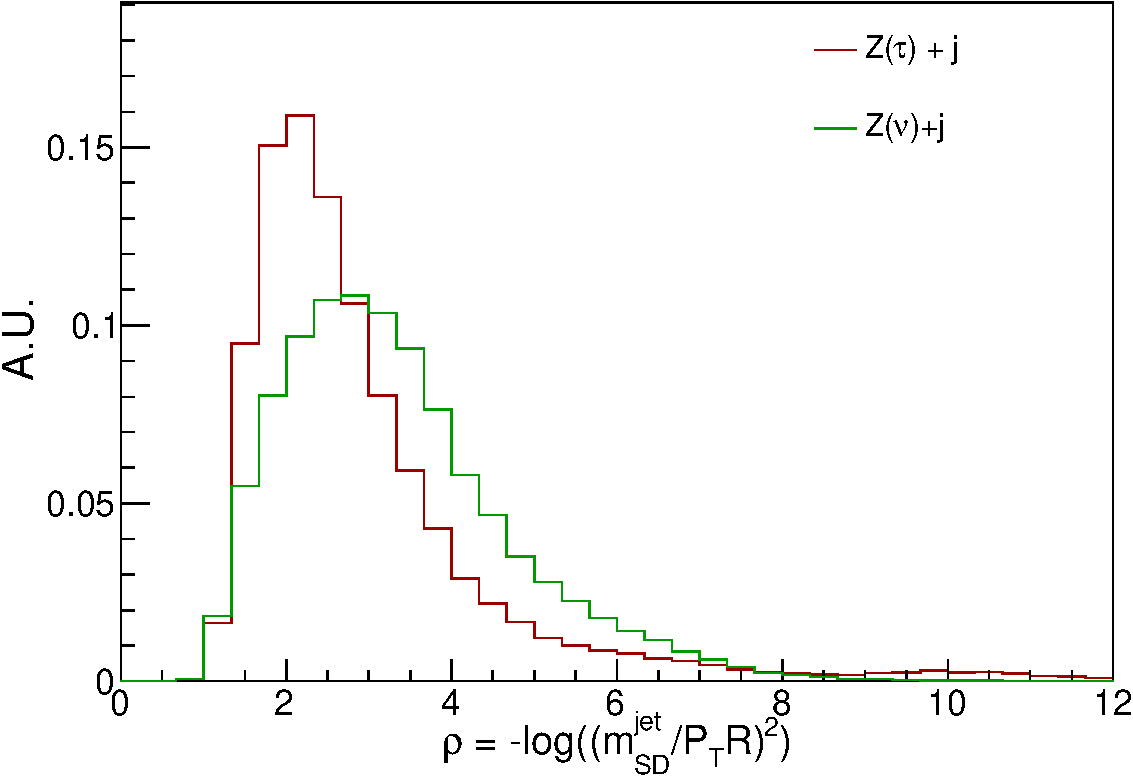
\includegraphics[width=0.7\textwidth]{Canv_jetrho.pdf}
        \caption{Variable $\rho$, a logarithmic function of soft drop mass and $P_{T}$ of the jet (distribution has been normalized to unit area under curve)}
    \end{center}
\end{figure}
\begin{figure}[H]
    \begin{center}
        \includegraphics[width=0.7\textwidth]{Canv_jetrsdmass.pdf}
        \caption{Soft drop mass of jet (in GeV) (distribution has been normalized to unit area under curve)}
    \end{center}
\end{figure}
\begin{figure}[H]
    \begin{center}
        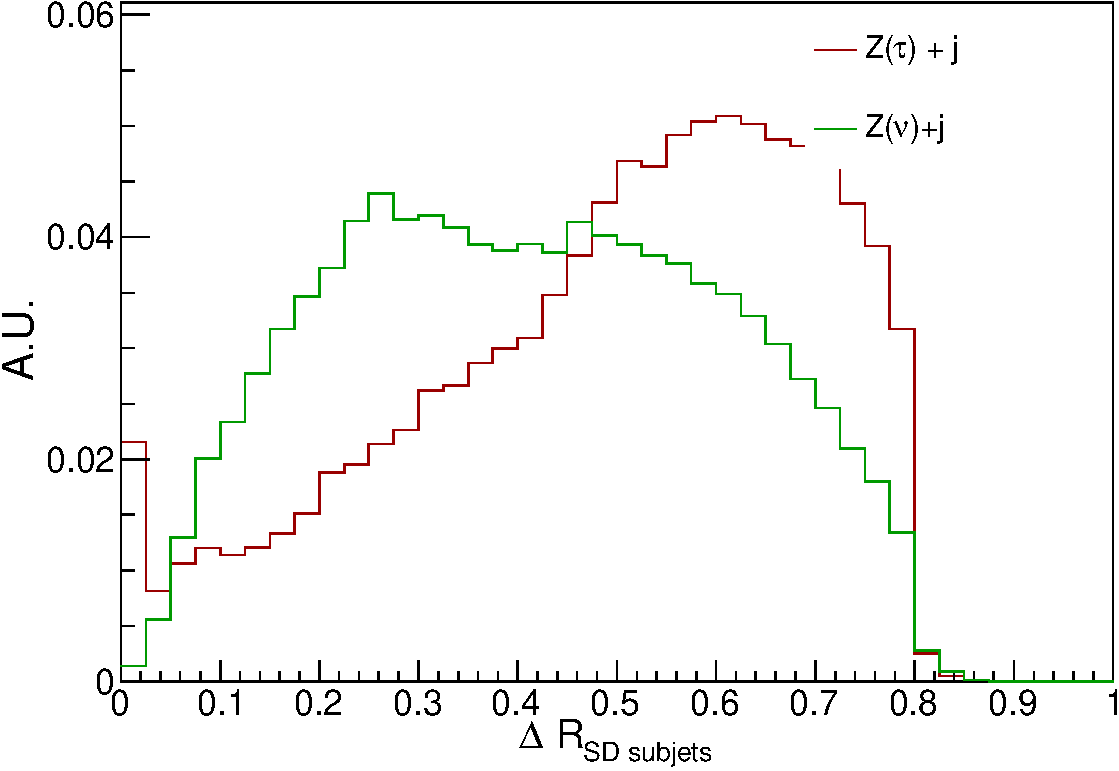
\includegraphics[width=0.7\textwidth]{Canv_jetsddelR.pdf}
        \caption{Separation between subjets of the soft dropped jet in rapidity-azimuth plane (distribution has been normalized to unit area under curve)}
    \end{center}
\end{figure}
\begin{figure}[H]
    \begin{center}
        \includegraphics[width=0.7\textwidth]{Canv_jettrackptrat.pdf}
        \caption{Ratio of $P_{T}$ of the leading track in the jet with respect to jet $P_{T}$ (distribution has been normalized to unit area under curve)}
    \end{center}
\end{figure}
\begin{figure}[H]
    \begin{center}
        \includegraphics[width=0.7\textwidth]{Canv_subjet1_corefrac.pdf}
        \caption{Energy fraction of the leading subjet inside a cone of $\Delta R=0.1$ around the subjet axis (distribution has been normalized to unit area under curve)}
    \end{center}
\end{figure}
\begin{figure}[H]
    \begin{center}
        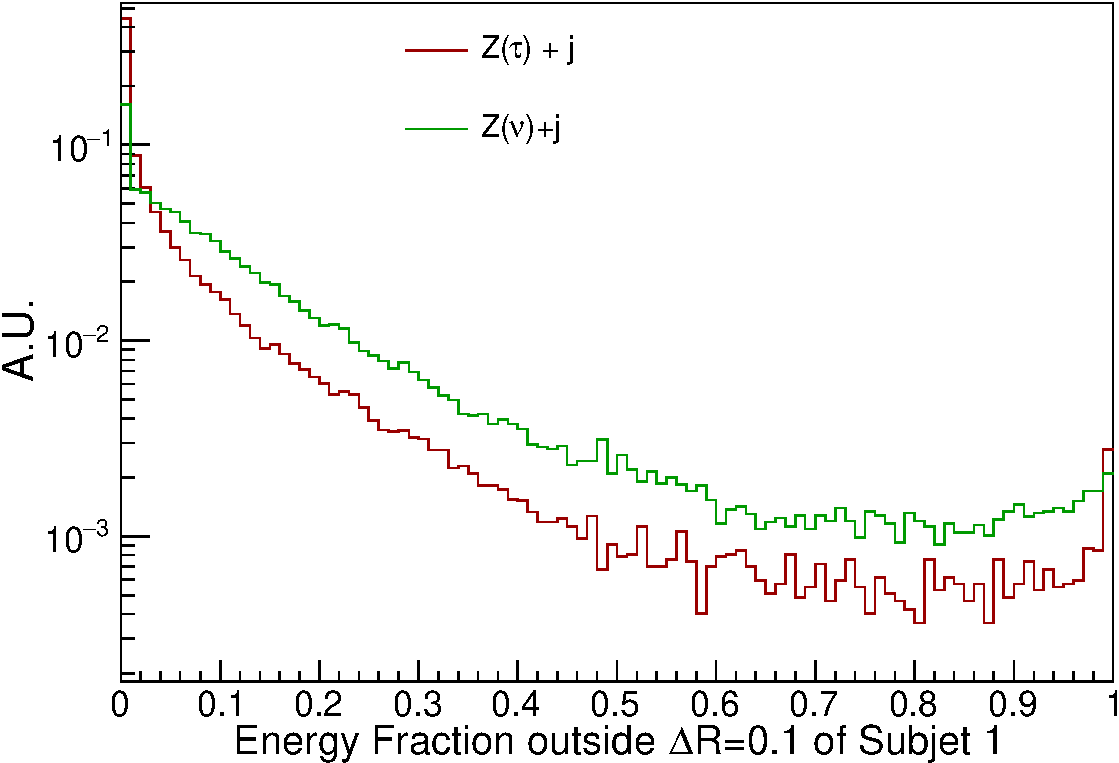
\includegraphics[width=0.7\textwidth]{Canv_subjet1_outfrac.pdf}
        \caption{Energy fraction of the leading subjet outside a cone of $\Delta R=0.1$ around the subjet axis (distribution has been normalized to unit area under curve)}
    \end{center}
\end{figure}
\begin{figure}[H]
    \begin{center}
        \includegraphics[width=0.7\textwidth]{Canv_subjet1_ptfrac.pdf}
        \caption{Ratio of leading subjet $P_{T}$ and jet $P_{T}$ (distribution has been normalized to unit area under curve)}
    \end{center}
\end{figure}
\begin{figure}[H]
    \begin{center}
        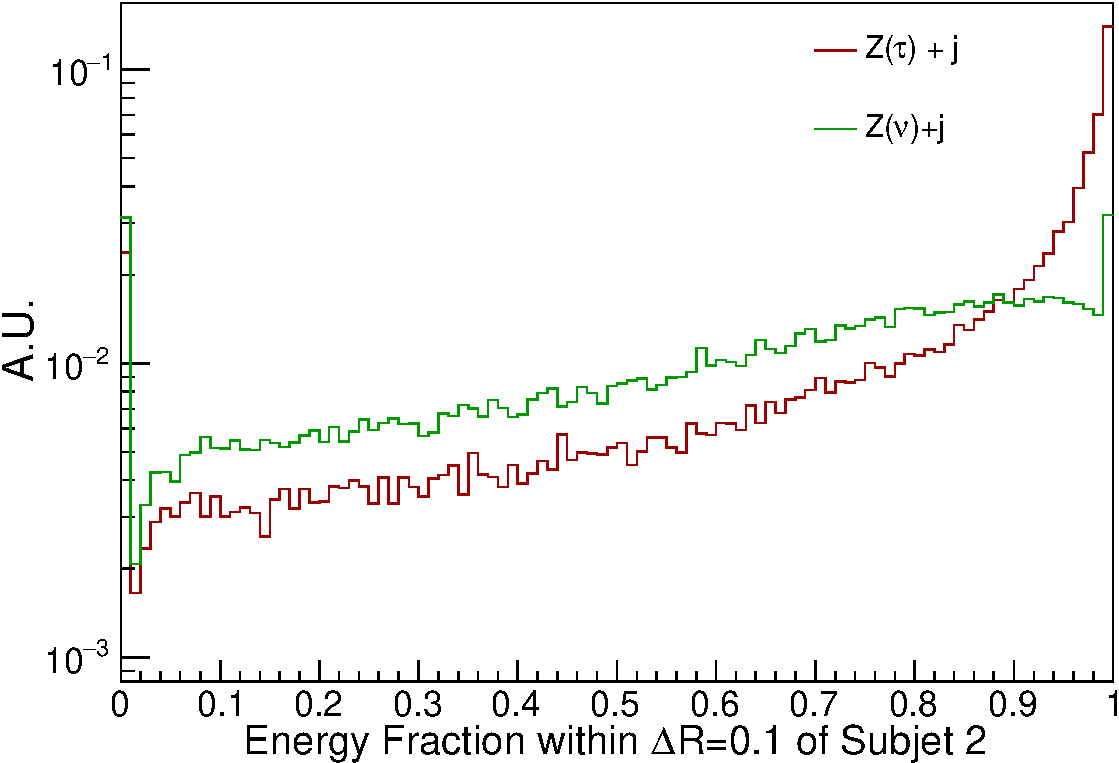
\includegraphics[width=0.7\textwidth]{Canv_subjet2_corefrac.pdf}
        \caption{Energy fraction of the subleading subjet inside a cone of $\Delta R=0.1$ around the subjet axis (distribution has been normalized to unit area under curve)}
    \end{center}
\end{figure}
\begin{figure}[H]
    \begin{center}
        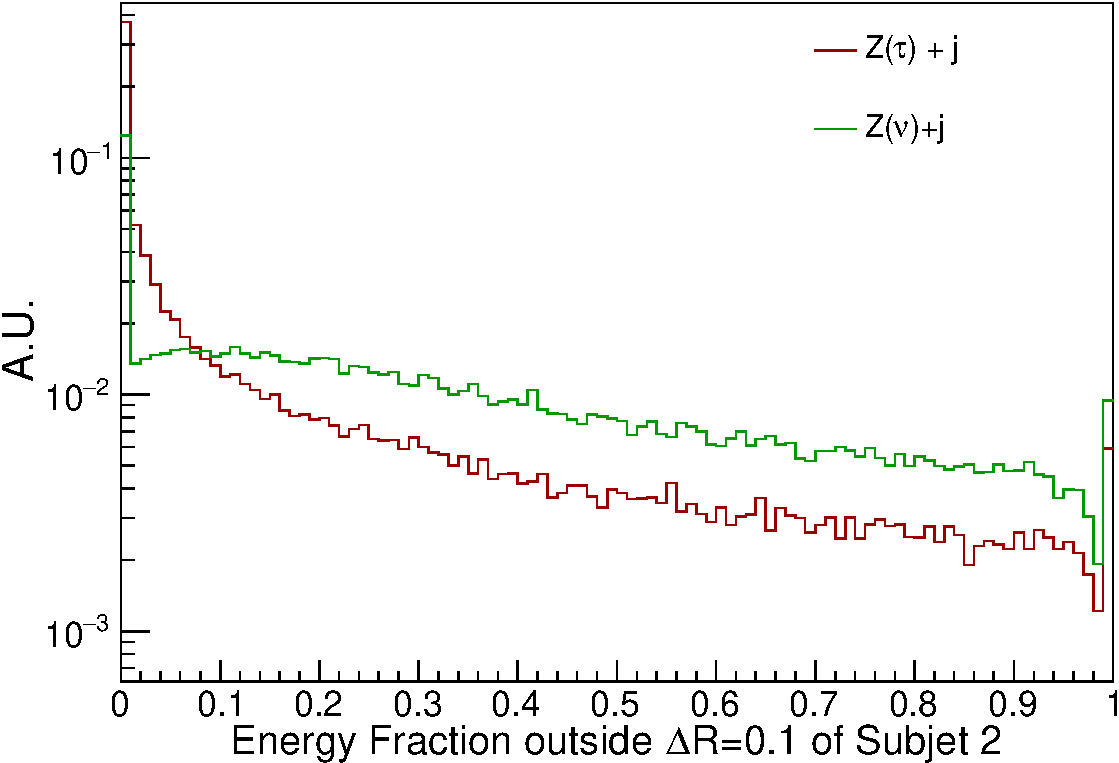
\includegraphics[width=0.7\textwidth]{Canv_subjet2_outfrac.pdf}
        \caption{Energy fraction of the subleading subjet outside a cone of $\Delta R=0.1$ around the subjet axis (distribution has been normalized to unit area under curve)}
    \end{center}
\end{figure}
\begin{figure}[H]
    \begin{center}
        \includegraphics[width=0.7\textwidth]{Canv_subjet2_ptfrac.pdf}
        \caption{Ratio of subleading subjet $P_{T}$ and jet $P_{T}$ (distribution has been normalized to unit area under curve)}
    \end{center}
\end{figure}
\begin{figure}[H]
    \begin{center}
        \includegraphics[width=0.7\textwidth]{Canv_subjets_ptfrac.pdf}
        \caption{Ratio of sum of $P_{T}$ of leading and subleading jet with respect to jet $P_{T}$ (distribution has been normalized to unit area under curve)}
    \end{center}
\end{figure}
\begin{figure}[H]
    \begin{center}
        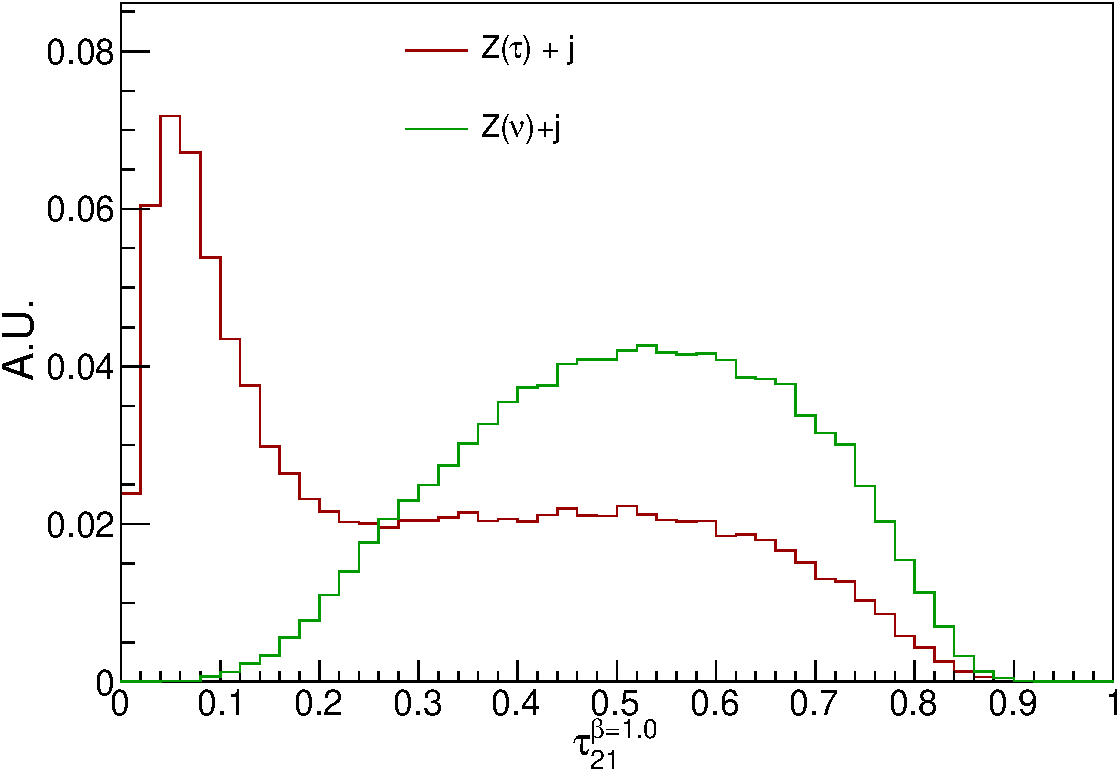
\includegraphics[width=0.7\textwidth]{Canv_tau21_b1.pdf}
        \caption{Subjettiness ratio $\tau_{21}$ for angular coefficient $\beta=1.0$ (distribution has been normalized to unit area under curve)}
    \end{center}
\end{figure}
\begin{figure}[H]
    \begin{center}
        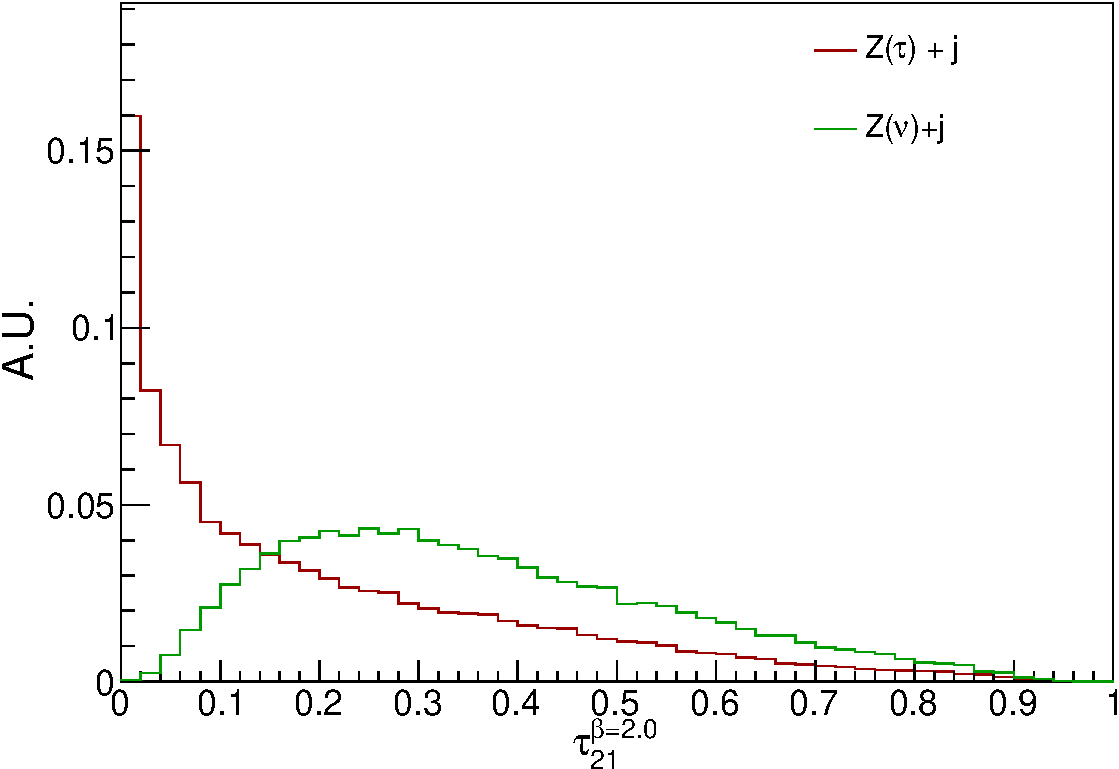
\includegraphics[width=0.7\textwidth]{Canv_tau21_b2.pdf}
        \caption{Subjettiness ratio $\tau_{21}$ for angular coefficient $\beta=2.$ (distribution has been normalized to unit area under curve)}
    \end{center}
\end{figure}
\begin{figure}[H]
    \begin{center}
        \includegraphics[width=0.7\textwidth]{Canv_tau21_bp5.pdf}
        \caption{Subjettiness ratio $\tau_{21}$ for angular coefficient $\beta=0.5$ (distribution has been normalized to unit area under curve)}
    \end{center}
\end{figure}
\begin{figure}[H]
    \begin{center}
        \includegraphics[width=0.7\textwidth]{Canv_tau32_b1.pdf}
        \caption{Subjettiness ratio $\tau_{32}$ for angular coefficient $\beta=1.$ (distribution has been normalized to unit area under curve)}
    \end{center}
\end{figure}
\begin{figure}[H]
    \begin{center}
        \includegraphics[width=0.7\textwidth]{Canv_tau32_b2.pdf}
        \caption{Subjettiness ratio $\tau_{32}$ for angular coefficient $\beta=2.$ (distribution has been normalized to unit area under curve)}
    \end{center}
\end{figure}
\begin{figure}[H]
    \begin{center}
        \includegraphics[width=0.7\textwidth]{Canv_tau32_bp5.pdf}
        \caption{Subjettiness ratio $\tau_{32}$ for angular coefficient $\beta=0.5$ (distribution has been normalized to unit area under curve)}
    \end{center}
\end{figure}
\begin{figure}[H]
    \begin{center}    
        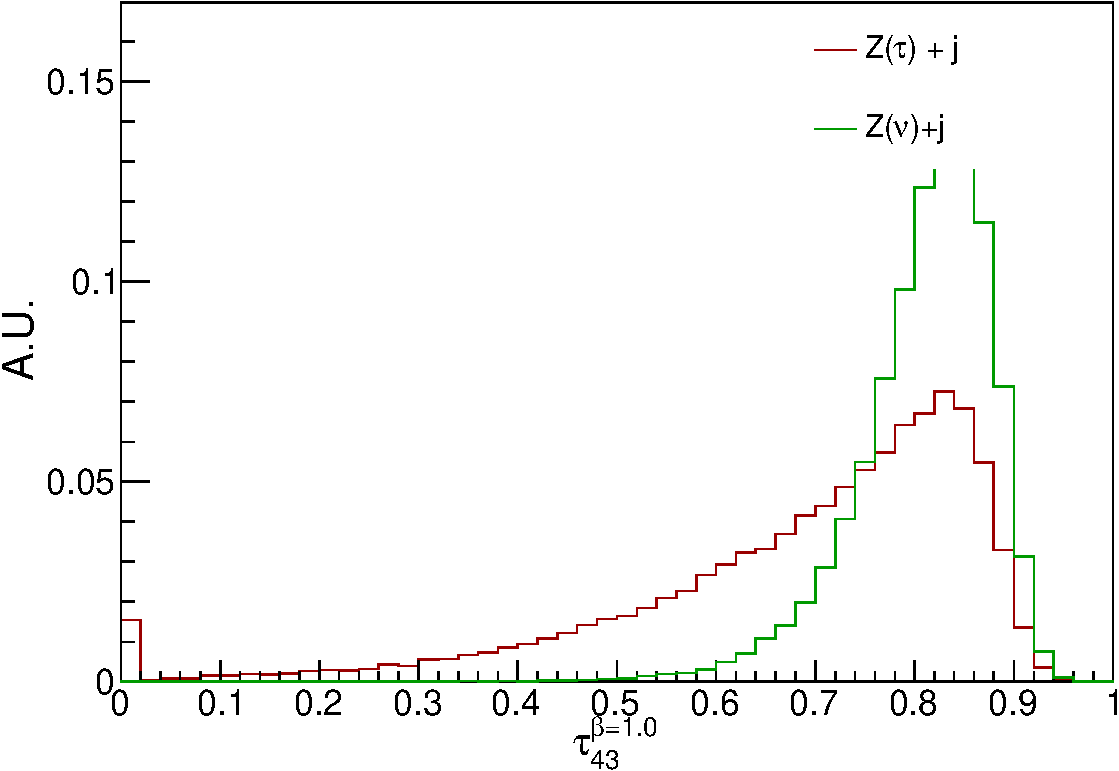
\includegraphics[width=0.7\textwidth]{Canv_tau43_b1.pdf}
        \caption{Subjettiness ratio $\tau_{43}$ for angular coefficient $\beta=1.$ (distribution has been normalized to unit area under curve)}
    \end{center}
\end{figure}
\begin{figure}[H]
    \begin{center}
        \includegraphics[width=0.7\textwidth]{Canv_tau43_b2.pdf}
        \caption{Subjettiness ratio $\tau_{43}$ for angular coefficient $\beta=2.$ (distribution has been normalized to unit area under curve)}
    \end{center}
\end{figure}
\begin{figure}[H]
    \begin{center}
        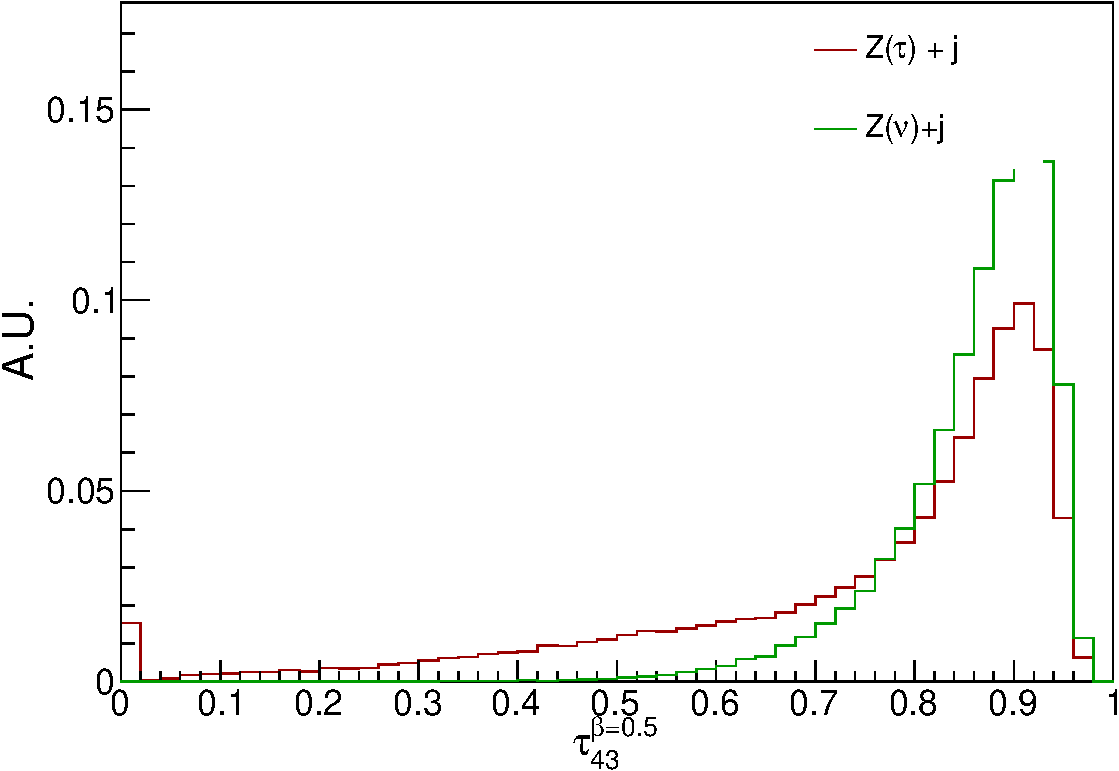
\includegraphics[width=0.7\textwidth]{Canv_tau43_bp5.pdf}
        \caption{Subjettiness ratio $\tau_{43}$ for angular coefficient $\beta=0.5$ (distribution has been normalized to unit area under curve)}
    \end{center}
\end{figure}